\documentclass{report}

\usepackage[a4paper, total={6in, 8in}, margin=1in,footskip=0.25in]{geometry} \usepackage{amsmath, amsthm, amssymb, booktabs, chemfig, graphicx, float, pgfplots, setspace, siunitx, tabularray} \usepackage{tabularray} \usepackage[hidelinks]{hyperref}

\renewcommand{\familydefault}{\sfdefault}

\setlength{\parindent}{0pt}
\setlength{\parskip}{0.8em}

\pgfplotsset{compat=1.18}

\graphicspath{ {.././Images/} }

\title{\Huge Year 12 Physics - Module 7}
\author{L. Cheung}

\tolerance=1
\emergencystretch=\maxdimen
\hyphenpenalty=10000
\hbadness=10000

\begin{document}
	\maketitle
	\tableofcontents
\newpage

\chapter{Investigations}

	\section{Investigation 1: Speed of Light Investigations}
	
		\textbf{Summarise the historical and contemporary methods used to determine the speed of light and explain its current relationship to the measurement of time and distance.}

			Galileo attempted to measure the speed of light by using lantern signals across a large distance and calculating the delay over the gap. However, varying human reflexes and the primitive time measuring equipment available inhibited any recordings taken.

			Later, Romer used the eclipses of Jupiter's moon Io to estimate the speed of light. Romer observed that the time between the eclipses was not constant. Using the assumption that the orbital period of Io was not changing, he deduced that the variation was due to changes in the difference in distance between Jupiter and Earth. From his observations, Romer found the speed of light to be 226,663 km/s, 24.4\% lower than its actual value.

			Fizeau used an experiment where a toothed wheel interfered with a light source that reflected off a mirror a great distance away. By adjusting the rotational velocity of the wheel, the reflected light may or may not have been reflected.

			Foucault's experiment used a similar setup, however used a rotating mirror instead of a toothed wheel. By analysing the angle between the light source and the light received, Foucault could determine the speed of light.

			\begin{align*}
				c &= \frac{d}{t} = \frac{d}{\frac{\Delta \theta}{\omega}} = \frac{d \omega}{\Delta \theta}
			\end{align*}

			Using Maxwell's discovery on electromagnetism in the 1860s, Rosa and Dorsey derived a formula using the electric permittivity and magnetic permeability constants to calculate the speed of light.

			\begin{align*}
				c = \frac{1}{\sqrt{\epsilon \mu}}
			\end{align*}

		
\newpage

	\section{Investigation 2: Spectral Analysis}
	
		\textbf{Aim}: To determine the emission spectra of various elements

		\subsubsection{Materials}
		
			\begin{itemize}
				\item Spectroscope
				\item Spectral lamps with:
					\begin{itemize}
						\item Hydrogen
						\item Helium
						\item Neon
						\item Oxygen
						\item Mercury
					\end{itemize}
				\item Spectral lamp support
				\item Spectral lamp power supply
			\end{itemize}

		\subsubsection{Risk Assessment}

			\begin{table}[H]
				\setstretch{1.25}
				\centering
				\begin{tabular}{p{7cm}|p{7cm}}
					\textbf{Hazard} & \textbf{Precaution} \\ \hline
					High voltage power pack & Turn off when not in use, do not touch contact points \\
					Cuts from glass & Check spectral lamp before use, keep away from edge of table to prevent dropping \\
					Burns from UV light & Don't observe directly, only view via spectrometer
					
				\end{tabular}
			\end{table}

		\subsubsection{Method}
			\begin{enumerate}
				\item Prepare spectral support and power supply at 400V
				\item Insert hydrogen spectral
				\item Use spectrometer to observe emission spectrum and record wavelengths using chart on spectrometer
				\item Repeat steps 2-3 with helium, neon, sulfur, and mercury
				\item Record results
			\end{enumerate}

		\subsubsection{Results}
			\begin{table}[H]
				\centering
				\setstretch{1.25}
				\begin{tabular}{p{3cm}|p{10cm}}
					\textbf{Element}	& \textbf{Result}			\\ \hline
					Hydrogen		& Bright pink				\\
					Helium			& Red, orange, yellow			\\
					Neon			& Red, orange				\\
					Oxygen			& Pale blue white			\\
					Mercury			& Blue-green				\\
				\end{tabular}
			\end{table}

\newpage

	\section{Investigation 3: Diffraction of Light}
	
		\textbf{Summarise your qualitative analysis of light diffraction, including the experimental setup, observations, and what these phenomena demonstrate about the wave properties of light.}

			Light diffraction is the spreading out of a wave when passing around an obstacle. The scattering process changes the direction of propagation and causes the diffracting object to act as a secondary source of propagation. The degree of this direction change depends on the obstacle's size relative to that of the wavelength.

			Waves passing through a slit a relative size to its wavelength experience diffraction that creates a repeating pattern with alternating bright and dark points. Huygen's wave model of light proposed that when a wave reaches an opening, its wavefront becomes many individual points each emitting their own wavelets. As a result, waves passing through a slit will propagate outwards from the slit.

			Diffraction through two slits creates two secondary wave sources that interact constructively or destructively to produce alternating minima and maxima of diffraction. The intensity of light decreases away from the centre line.

			Young's double slit experiment involved passing a monochromatic light source through two narrow slits separated by a given distance. The results supported the wave model of light, where a particle based model could not account for the pattern produced.
				
			\begin{figure}[H]
				\centering
				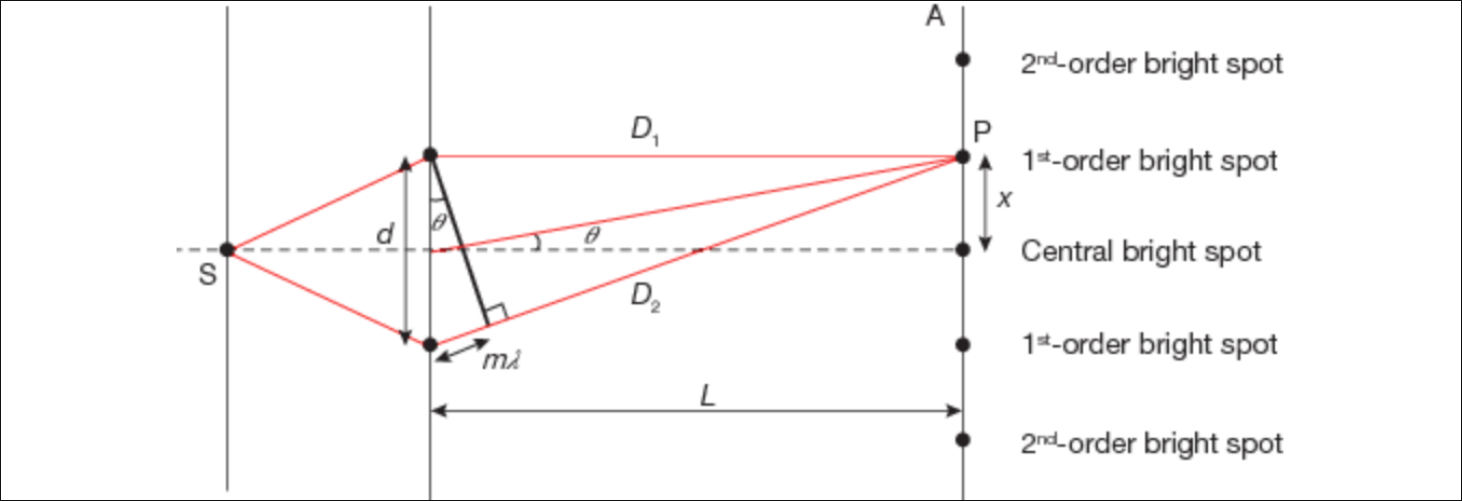
\includegraphics[width=15cm]{young_double_slit.png}
			\end{figure}


\newpage

	\section{Investigation 4: Interference and Diffraction}

		\textbf{Aim}: To observe the diffraction and interference of light using diffraction gratings
		\subsubsection{Materials}

			\begin{itemize}
				\item Laser pointer
				\item A diffraction grating set
				\item Meter ruler or tape measure
			\end{itemize}

		\subsubsection{Risk Assessment}
		
			\begin{table}[H]
				\setstretch{1.25}
				\centering
				\begin{tabular}{p{7cm}|p{7cm}}
					\textbf{Hazard} & \textbf{Precaution} \\ \hline
					Retina burns & Do not directly look at laser light \\
					Dropping equipment & Handle with caution, keep secure on table

				\end{tabular}
			\end{table}
		
		\subsubsection{Method}

			\begin{enumerate}
				\item Use supports such as retort stands to set up the laser pointer so that it shines perpendicularly onto a screen, wall, or board at least one meter away.
				\item Mount the diffraction grating directly in front of the laser pointer so that a regular row of dots appears on the screen.
				\item Measure the values of $x$ and $L$, and record these in your results table, along with the $N$ value for your grating.
				\item Repeat this procedure for each grating of different $N$ value.
				\item Analyse the data to determine the wavelength of the laser pointer.
			\end{enumerate}

		\subsubsection{Results}

			\begin{table}[H]
				\centering
				\setstretch{1.25}
				\begin{tabular}{p{4cm}|p{2cm}|p{2cm}|p{2cm}|p{2cm}}
					Slit separation $d$ (m)		& $x$ (m)	& L (m)		& $\lambda$ (m) 		& $\lambda$ (nm)	\\ \hline
					$100 \times 10^{-6}$		& 0.034		& 5.44		& $6.25 \times 10^{-7}$		& 625			\\
					$200 \times 10^{-6}$		& 0.016		& 5.44		& $5.88 \times 10^{-7}$		& 588			\\
					$300 \times 10^{-6}$		& 0.011		& 5.44		& $6.07 \times 10^{-7}$		& 607			\\
				\end{tabular}
			\end{table}
			
			Slit separation 1
			\begin{align*}
				\text{At very small angles, } \sin{\theta} = \tan{\theta} \\
				d \sin{\theta} &= m \lambda \\
				\sin{\theta} = \frac{m \lambda}{d} &= \frac{x}{L} \\
				\lambda &= \frac{dx}{L} \\
					&= \frac{100 \times 10^{-6} \times 0.034}{5.44} \\
					&= 6.25 \times 10^{-7} \\
			\text{Actual $\lambda$ of Ne-He laser} &= 6.328 \times 10^{-7}
			\end{align*}

			Slit separation 2
			\begin{align*}
				d \sin{\theta} &= m \lambda \\
				\sin{\theta} = \frac{m \lambda}{d} &= \frac{x}{L} \\
				\lambda &= \frac{dx}{L} \\
					&= \frac{200 \times 10^{-6} \times 0.016}{5.44} \\
					&= 5.88 \times 10^{-7} \\
			\text{Actual $\lambda$ of Ne-He laser} &= 6.328 \times 10^{-7}
			\end{align*}

			Slit separation 3
			\begin{align*}
				d \sin{\theta} &= m \lambda \\
				\sin{\theta} = \frac{m \lambda}{d} &= \frac{x}{L} \\
				\lambda &= \frac{dx}{L} \\
					&= \frac{300 \times 10^{-6} \times 0.011}{5.44} \\
					&= 6.07 \times 10^{-7} \\
				\text{Actual $\lambda$ of Ne-He laser} &= 6.328 \times 10^{-7}
			\end{align*}

\newpage

	\section{Investigation 5: Polarisation and Malus's Law}
	
		\textbf{Aim}: To observe plane polarisation of light using polarising filters, and to verify Malus' Law

		\subsubsection{Materials}
		
			\begin{itemize}
				\item Torch
				\item Lux meter
				\item 2 polarising filters
				\item A protractor
				\item Retort stand
				\item Bosshead
				\item Clamp
			\end{itemize}

		\subsubsection{Risk Assessment}
		
			\begin{table}[H]
				\centering
				\setstretch{1.25}
				\begin{tabular}{p{7cm}|p{7cm}}
					\textbf{Hazard}			& \textbf{Precaution}		\\ \hline
					Eye damage from torch		& Do not look directly at light source \\
					Burning				& Do not touch torch when in use. Allow cooling time when necessary
				\end{tabular}
			\end{table}

		\subsubsection{Method}
			
			\begin{enumerate}
				\item Attach polarising filters to retort stand using bosshead
				\item Attach torch above the polarising filters using bosshead and clamp facing down
				\item Place lux meter below the polarising filter, lining up with the torch
				\item Remove external light sources
				\item Record the lux where the polarising filters have angles of 0, 30, 45, 60, 90 degrees.
			\end{enumerate}

		\subsubsection{Results}
		
			\begin{table}[H]
				\centering
				\setstretch{1.25}
				\begin{tabular}{p{6cm}|p{5cm}|p{5cm}}
					\textbf{Angle between filters (degrees)}& \textbf{Measured intensity (lux)}	& \textbf{Calculated Intensity (lux)}		\\ \hline
					0					& 175					& 175					\\
					30					& 132					& 131					\\
					45					& 91					& 87.5					\\
					60					& 57					& 43.8					\\
					90					& 20					& 0					\\
				\end{tabular}
			\end{table}

			\begin{figure}[H]
				\centering
				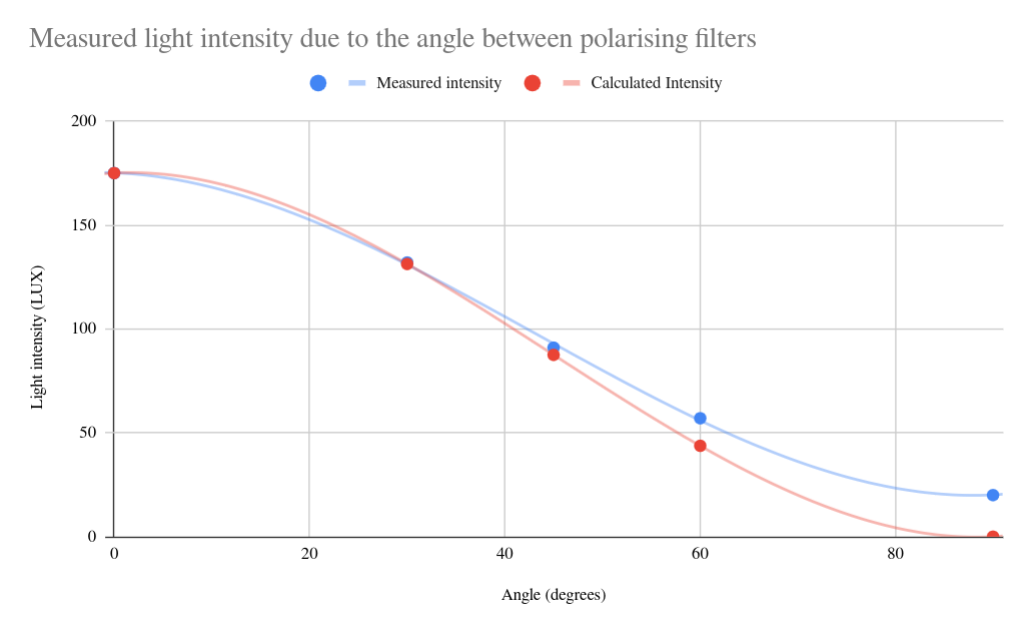
\includegraphics[width=15cm]{prac_5_graph.png}
			\end{figure}

\newpage

\chapter{Review Questions}

	\section{Electromagnetic Spectrum}
		\begin{enumerate}
			\item B
			\item D
			\item B
			\item C
			\item A
			\item \textbf{Figure 8.11 shows the emission spectrum of sodium}
				\begin{enumerate}
					\item \textbf{Describe an experiment that could be used to examine the emission spectrum of an element.}
						\subitem The spectral lamp experiment can be used to observe the emission spectrum of an element. Running high voltage current through a spectral lamp containing a specific element will emit a bright spectrum that can be split into wavelengths by a prism or a spectrocope.

					\item \textbf{Explain how emission spectra can be used to identify the elements in a sample?}
						\subitem A complete emission spectra can be analysed to find the lines in the black body spectrum and comparing that with the spectra of known elements.

					\item \textbf{If sodium was present in the atmosphere of the Sun, how would it affect the emission spectra of the Sun?}
						\subitem If sodium is present, the Sun's emission spectrum will have lines at 589 nm to 590 nm.
				\end{enumerate}

			\item \textbf{Outline one method that has been used to measure the speed of light}
				\subitem The speed of light light has been measured by Hertz who used an induction coil to produce a spark of a particular frequency. A spark gap was placed such that it would interact with the produced electromagnetic waves. By adjusting the position of the spark gap to maximise its intensity, the wavelength can be measured. Then, the formula $v=f \lambda$ can be used to determine the velocity of light.

			\item \textbf{About half of the visible stars in the sky are binary star systems, which consist of two stars orbiting each other. Consider two stars of similar mass in a binary system that has its orbital plane almost parallel to the line of sight from the Earth. Each of the hydrogen atomic absorption lines in the stellar spectrum of the binary star system are observed to split into two lines of slightly different frequency and recombine to a single line every four days.}

				\begin{enumerate}
					\item \textbf{Explain why the motion of the stars would cause the atomic absorption lines in the stellar spectra to change in this way.}
						\subitem The light from the stars will become red or blue shifted depending on each star's velocity relative to the viewer. As the hydrogen atomic absorption lines split, the stars rotate out of alignment with the Earth. One star moves away from the Earth, becoming redshifted and resulting in a longer wavelength, whereas the other star moves towards the Earth and its emitted light becomes blueshifted. When the stars are travelling perpendicularly to the Earth, ie. they are in alignment with the Earth, there is no relative motion and hence no red or blue shifting effect, creating a single line on the spectrum.

					\item \textbf{Determine the orbital period of this binary star system.}
						\subitem 8 days.

					\item \textbf{Explain why some non-hydrogen absorption lines from the binary system move back and forth around a specific frequency periodically but do not split and recombine like the hydrogen lines.}
						\subitem In order for the absorption line to split, the element blocking the wavelength must be present in both stars. If it only present in one star, then a single line will be observed, shifting as it is red or blue shifted.
				\end{enumerate}

			\item \textbf{Maxwell used his equations of electromagnetism to predict the existence of electromagnetic waves.}

				\begin{enumerate}
					\item \textbf{Explain how an electromagnetic wave can be produced.}
						\subitem An electromagnetic wave can be produced by oscillating charged particles. This creates a change in electric field that produces a change in magnetic field that is perpendicular to the charge movement.

					\item \textbf{Describe the structure of electromagnetic waves in terms of electric and magnetic fields.}
						\subitem Electromagnetic waves consist of electric and magnetic fields travelling perpendicular to each other.

					\item \textbf{If the source of an electromagnetic wave was removed, would the existing waves produced by the source continue to propagate? Justify your answer.}
						\subitem If the source is removed, the electromagnetic wave will continue to move. This is due to electromagnetic waves being self-propagating as the change in magnetic and electric fields cause each other.
				\end{enumerate}

			\item \textbf{Explain how an examination of the light from a star can be used to provide information on three physical properties of the star.}

				\subitem The gaps in the absorption spectrum of a star can show what elements are present in the star. A star's nucleus produces all wavelengths of light, however some are absorbed by the elements in the star and become gaps in the spectrum that can be analysed to determine the chemical composition of the star.

				The translational velocity of a star can also be determined by observing red and blue shifting patterns in the spectrum. The line will appear to move left and right, and this change in wavelength can be used to calculated velocity relative to the Earth and hence translational velocity.

				If the star has high density, more collisions occur between atoms and furthermore between electrons. This produces variations in energy of the electrons that blurs the lines on the absorption spectrum.
		\end{enumerate}

\end{document}

